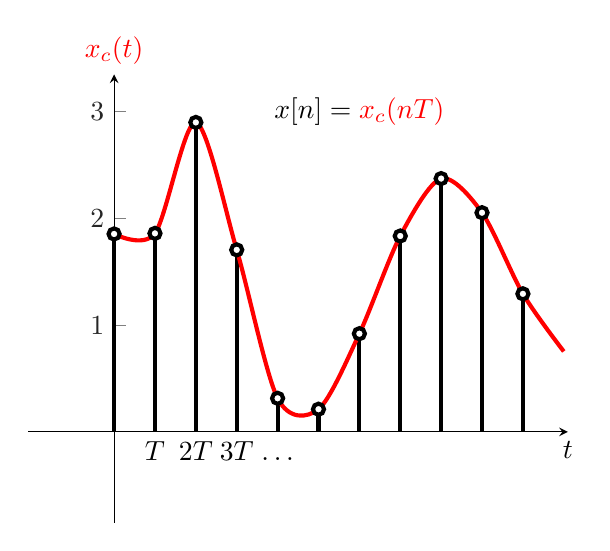
\begin{tikzpicture} 
\begin{axis}[
axis lines*=middle,
enlargelimits = true,
xmin=-1,
xmax=10,
ymin=-0.5,
ymax=3,
axis line style={->,>=stealth},
xlabel={$t$},
ylabel={$\textcolor{red}{x_c(t)}$},
%yticklabel style = {yshift=0.2cm},
every axis x label/.style={
    at={(ticklabel* cs:1)},
    anchor=north,
},
every axis y label/.style={
    at={(ticklabel* cs:1)},
    anchor=south,
},
xtick={0, 1, ..., 3},
%ytick={1},
%xtick={-3.14, -1, 1, 3.14},
xticklabels={0, $T$, $2T$, $3T$},
%xmajorgrids,
%ymajorgrids,
every outer y axis line/.append style={white!15!black},
every y tick label/.append style={font=\color{white!15!black}},
legend style={draw=white!15!black,fill=white,legend cell align=left}]

\pgfmathsetseed{103}
\addplot[ycomb, mark=*, line width=2pt, domain=0:10, samples=11, line width=1.5, mark options={scale=1,fill=white}] {sin(deg(x)) + 0.5*rand + 1.5};
\pgfmathsetseed{103}
\addplot[red, smooth, line width=2pt, domain=0:11, samples=12, line width=1.5] {sin(deg(x)) + 0.5*rand + 1.5};
\node (dots) at (axis cs: 4, -0.25) {$\ldots$};
\node at (axis cs: 6, 3) {$x[n] = \textcolor{red}{x_c(nT)}$};
\end{axis}
\end{tikzpicture}
